\documentclass[aspectratio=169]{beamer}
\usepackage{graphicx}
\usepackage{tikz}
\usepackage{amsmath}
\usetikzlibrary{arrows.meta,positioning,fit,calc}

\setbeamertemplate{navigation symbols}{}
\setbeamertemplate{footline}[frame number]
\setbeamerfont{frametitle}{size=\Large}

\title{Teaching a Super-Resolution Model to Grow Subhalos}
\subtitle{Directly fine-tuning SR2 for the small-scale structure it misses}
\author{}
\date{}

\begin{document}

% ======================================================================
%  BACKGROUND
% ======================================================================

\begin{frame}
\titlepage
\end{frame}

% ----------------------
\begin{frame}{What is a dark-matter simulation?}
\small
\begin{columns}[T]
\column{0.42\textwidth}
\begin{itemize}
    \item The universe's matter is represented by many \textbf{particles}.
    \item Gravity pulls them together over cosmic time; they clump into
          \textbf{halos} and \textbf{filaments} --- the ``cosmic web''.
    \item A simulation just tracks where every particle \emph{starts} and
          where gravity \emph{moves} it.
\end{itemize}
\vspace{0.2cm}
{\footnotesize We work in the \textbf{Lagrangian} picture: particles begin on a
regular grid, and the model predicts each one's \textbf{displacement}.}

\column{0.58\textwidth}
\centering
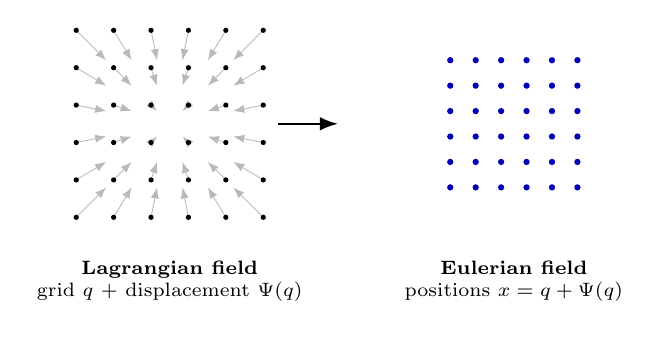
\begin{tikzpicture}[scale=0.95]
\coordinate (C) at (1.25,1.25);
% --- Panel A: Lagrangian grid + displacement field ---
\begin{scope}
  \foreach \i in {0,1,2,3,4,5}{
    \foreach \j in {0,1,2,3,4,5}{
      \coordinate (P) at (\i*0.5,\j*0.5);
      \draw[-{Latex[length=1.4mm]},gray!55,line width=0.3pt] (P)--($(P)!0.32!(C)$);
      \fill[black] (P) circle (1.0pt);
    }
  }
  \node[below,align=center,font=\scriptsize] at (1.25,-0.45)
    {\textbf{Lagrangian field}\\grid $q$ + displacement $\Psi(q)$};
\end{scope}
% --- Panel B: Eulerian result ---
\begin{scope}[xshift=4.6cm]
  \coordinate (C2) at (1.25,1.25);
  \foreach \i in {0,1,2,3,4,5}{
    \foreach \j in {0,1,2,3,4,5}{
      \coordinate (P) at (\i*0.5,\j*0.5);
      \fill[blue!70!black] ($(P)!0.32!(C2)$) circle (1.2pt);
    }
  }
  \node[below,align=center,font=\scriptsize] at (1.25,-0.45)
    {\textbf{Eulerian field}\\positions $x=q+\Psi(q)$};
\end{scope}
\draw[-{Latex},thick] (2.7,1.25)--(3.5,1.25);
\end{tikzpicture}

{\footnotesize The density we see is just \emph{where the moved particles pile
up}: $\;\delta=\mathrm{CIC}(q+\Psi)$. Get the displacement right and the density
follows.}
\end{columns}
\end{frame}

% ----------------------
\begin{frame}{Motivation: HR simulations are expensive}
\begin{columns}
\column{0.52\textwidth}
\begin{itemize}
    \item Cosmological simulations need large volume \emph{and} high resolution.
    \item HR simulations resolve small-scale structure, but are expensive.
    \item LR simulations are cheaper, but miss small-scale information.
    \item Goal: use ML to recover HR-like structure from LR data.
\end{itemize}
\[
x_{\mathrm{LR}} \rightarrow x_{\mathrm{HR}}
\]
\column{0.48\textwidth}
\includegraphics[width=\textwidth]{cost.png}
\end{columns}
\end{frame}

% ----------------------
\begin{frame}{What is super-resolution here?}
\begin{columns}
\column{0.50\textwidth}
\includegraphics[width=\textwidth]{lr_hr_sr_label.png}
\includegraphics[width=\textwidth]{lr_hr_sr.png}
\column{0.50\textwidth}
\begin{itemize}
    \item Input: low-resolution simulation output.
    \item Output: high-resolution / super-resolved field.
    \item Objects: density, displacement, particle positions.
\end{itemize}
\[
G_\theta(x_{\mathrm{LR}}, z) = \hat{x}_{\mathrm{HR}}
\]
\end{columns}
\end{frame}

% ======================================================================
%  SR2
% ======================================================================

\begin{frame}{SR2: the model we build on}
\small
\begin{columns}[T]
\column{0.54\textwidth}
\begin{itemize}
    \item A \textbf{GAN} with a U-Net generator.
    \item Operates on the \textbf{Lagrangian displacement} field.
    \item Two critics, so it is judged on \emph{both} views:
    \begin{itemize}
        \item the \textbf{Lagrangian} displacement field, and
        \item the \textbf{Eulerian} density field.
    \end{itemize}
    \item Paired training: LR $\rightarrow$ HR with real HR supervision.
\end{itemize}
\column{0.46\textwidth}
\centering
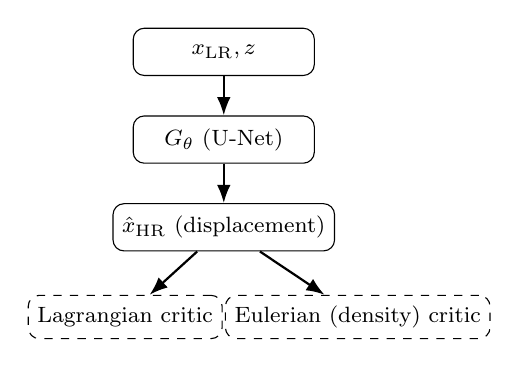
\begin{tikzpicture}[
    node distance=0.5cm,
    box/.style={draw, rounded corners, minimum width=2.3cm, minimum height=0.6cm, align=center, font=\footnotesize},
    crit/.style={draw, rounded corners, dashed, minimum width=2.3cm, minimum height=0.55cm, align=center, font=\footnotesize},
    arrow/.style={-{Latex}, thick}
]
\node[box] (lr) {$x_{\mathrm{LR}},z$};
\node[box, below=of lr] (g) {$G_\theta$ (U-Net)};
\node[box, below=of g] (hr) {$\hat{x}_{\mathrm{HR}}$ (displacement)};
\node[crit, below left=0.55cm and -1.4cm of hr] (cl) {Lagrangian critic};
\node[crit, below right=0.55cm and -1.4cm of hr] (ce) {Eulerian (density) critic};
\draw[arrow] (lr)--(g);
\draw[arrow] (g)--(hr);
\draw[arrow] (hr)--(cl);
\draw[arrow] (hr)--(ce);
\end{tikzpicture}
\end{columns}
\end{frame}

% ----------------------
\begin{frame}{SR2 strength: field statistics essentially match HR}
\small
\begin{columns}[T]
\column{0.46\textwidth}
\centering
\begin{tabular}{l c}
\hline
Full-box metric & SR2 \\
\hline
Density high-$k$ $P/P_{\mathrm{HR}}$ & \textbf{0.977} \\
Density $\sigma/\sigma_{\mathrm{HR}}$ & \textbf{1.000} \\
\hline
\end{tabular}

\vspace{0.25cm}
{\footnotesize $P(k)$ = power spectrum: how much variance sits at spatial scale
$k$; high $k$ = small scales.}

\column{0.54\textwidth}
\includegraphics[width=\textwidth]{lr_hr_sr.png}
\end{columns}

\vspace{0.25cm}
\begin{block}{}
By the usual \emph{distribution-level} rulers, SR2 already looks essentially
perfect.
\end{block}
\end{frame}

% ----------------------
\begin{frame}{SR2 weakness we attack: it does not build subhalos sharply}
\small
A subhalo is a \textbf{sharp density peak}. SR2 puts \emph{some} mass in the
right region but leaves it \textbf{too smooth} to be a real, detectable object.

\centering
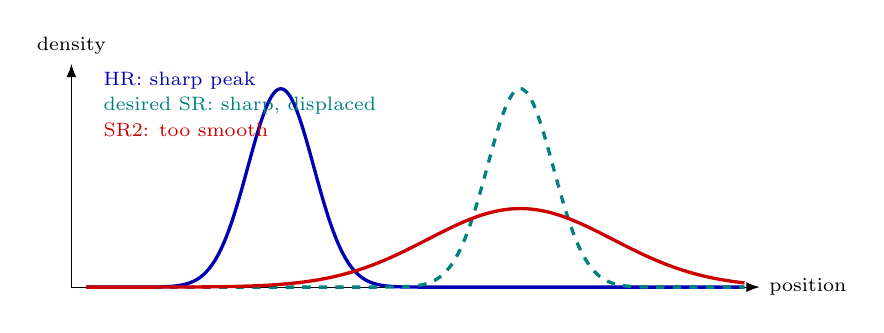
\begin{tikzpicture}[yscale=1.05,xscale=1.9]
% axes
\draw[-{Latex}] (-2.2,0)--(2.4,0) node[right,font=\scriptsize] {position};
\draw[-{Latex}] (-2.2,0)--(-2.2,2.7) node[above,font=\scriptsize] {density};
% HR: sharp bell at x=-0.8
\draw[very thick, blue!70!black, domain=-2.1:2.3, samples=140, smooth]
   plot (\x,{2.4*exp(-(\x+0.8)^2/(2*0.22*0.22))});
% Expected SR: sharp bell, displaced to x=+0.8
\draw[very thick, teal, dashed, domain=-2.1:2.3, samples=140, smooth]
   plot (\x,{2.4*exp(-(\x-0.8)^2/(2*0.22*0.22))});
% SR2: broad low bell at same displaced center x=+0.8
\draw[very thick, red!80!black, domain=-2.1:2.3, samples=140, smooth]
   plot (\x,{0.95*exp(-(\x-0.8)^2/(2*0.62*0.62))});
% legend
\node[blue!70!black,font=\scriptsize,anchor=west] at (-2.05,2.5) {HR: sharp peak};
\node[teal,font=\scriptsize,anchor=west]          at (-2.05,2.2) {desired SR: sharp, displaced};
\node[red!80!black,font=\scriptsize,anchor=west]  at (-2.05,1.9) {SR2: too smooth};
\end{tikzpicture}

{\footnotesize The peak may sit at the \emph{wrong position} --- that is fine and
unavoidable, because the exact location is \textbf{not recoverable} from the LR
field. What we need is a peak that is \emph{equally sharp}, not equally placed.}
\end{frame}

% ----------------------
\begin{frame}{The consequence, in numbers}
\small
\begin{columns}[T]
\column{0.40\textwidth}
\centering
\vspace{0.2cm}
{\Large \textbf{$\sim45\%$}}\\[0.15cm]
of HR subhalos are recovered by SR2.
\column{0.60\textwidth}
\centering
\begin{tabular}{r r r r}
\hline
$M_{\mathrm{host}}\,[M_\odot/h]$ & HR $\langle N_{\mathrm{sub}}\rangle$
& SR2 & SR2/HR \\
\hline
$1.00\times10^{12}$ & 4.9   & 4.0  & 0.81 \\
$3.16\times10^{12}$ & 14.1  & 6.8  & 0.48 \\
$1.00\times10^{13}$ & 44.0  & 11.5 & 0.26 \\
$3.16\times10^{13}$ & 125.4 & 13.8 & 0.11 \\
$1.00\times10^{14}$ & 337.6 & 17.3 & \alert{0.05} \\
\hline
\end{tabular}
\end{columns}

\vspace{0.35cm}
\begin{block}{Occupation saturation}
HR occupation rises steeply with host mass; SR2 saturates near $\sim$17 subhalos
per host. The failure is \emph{worst} in exactly the rich hosts that should
contain the most substructure.
\end{block}
\end{frame}

% ======================================================================
%  WHY IS IT HARD
% ======================================================================

\begin{frame}{Why is this hard?}
\small
A subhalo is not ``a bit more density'' --- it is a set of particles that are
\textbf{highly correlated with each other}: they must gather around a common
centre and stay gravitationally \textbf{bound}.

\vspace{0.15cm}
\textbf{One concrete requirement it must satisfy} --- balance spatial density
against velocity dispersion:
\begin{itemize}
    \item \textbf{Dense enough} (and not too hot) to form a bound halo \emph{at all}.
    \item \textbf{Denser / more coherent than its host background}, so a halo
          finder can pick it out from the surrounding host particles.
\end{itemize}

\vspace{0.2cm}
\centering
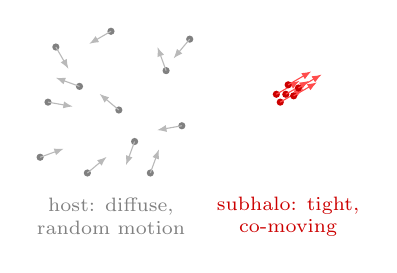
\begin{tikzpicture}[scale=1.0]
% host: scattered dots, random arrows
\foreach \x/\y/\a in {0/0.2/20, 0.5/1.1/160, 1.2/0.4/250, 0.2/1.6/300,
   1.6/1.3/110, 0.9/1.8/210, 1.4/0.0/70, 0.1/0.9/350, 1.0/0.8/140,
   1.8/0.6/190, 0.6/0.0/40, 1.9/1.7/230}{
   \fill[gray] (\x,\y) circle (1.3pt);
   \draw[-{Latex[length=1.2mm]},gray!55] (\x,\y)--++(\a:0.32);
}
% subhalo: tight cluster, coherent arrows
\foreach \x/\y in {3.0/1.0, 3.15/1.12, 3.05/0.9, 3.22/0.98, 3.12/1.0, 3.28/1.08}{
   \fill[red!80!black] (\x,\y) circle (1.3pt);
   \draw[-{Latex[length=1.2mm]},red!70] (\x,\y)--++(30:0.34);
}
\node[gray,font=\scriptsize,align=center] at (0.9,-0.55) {host: diffuse,\\random motion};
\node[red!80!black,font=\scriptsize,align=center] at (3.15,-0.55) {subhalo: tight,\\co-moving};
\end{tikzpicture}

\begin{block}{Why the GAN misses it}
Subhalos are a \emph{tiny fraction} of all particles, so this fine correlation
is \textbf{overlooked by the critic}, which is dominated by the far coarser
correlations of the large halos and the smooth field.
\end{block}
\end{frame}

% ======================================================================
%  METHOD
% ======================================================================

\begin{frame}{Method: masked direct fine-tuning of the SR2 generator}
\small
\begin{columns}[T]
\column{0.50\textwidth}
\begin{itemize}
    \item Take the frozen SR2 \textbf{generator} and fine-tune it \emph{directly}
          (no new generator, no adversary).
    \item Apply a differentiable \textbf{subhalo loss} only where it belongs:
          \textbf{mask} the gradient to the particles that HR says form
          subhalos.
    \item Everything else is left to the original SR2 objective, so global
          fidelity is preserved.
\end{itemize}
\vspace{0.15cm}
{\footnotesize The loss is normalised to \textbf{HR's own value} on each set, so
it can never ask for \emph{more} structure than HR has.}
\column{0.50\textwidth}
\centering
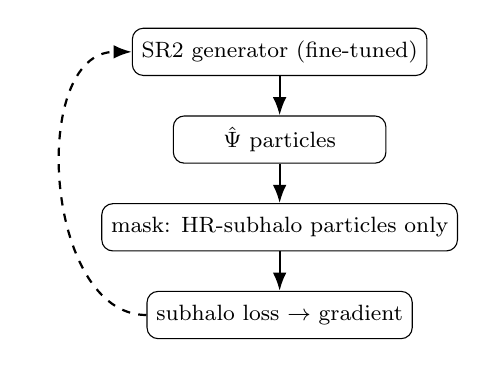
\begin{tikzpicture}[
    node distance=0.5cm,
    box/.style={draw, rounded corners, minimum width=2.7cm, minimum height=0.6cm, align=center, font=\footnotesize},
    arrow/.style={-{Latex}, thick}
]
\node[box] (g) {SR2 generator (fine-tuned)};
\node[box, below=of g] (out) {$\hat\Psi$ particles};
\node[box, below=of out] (mask) {mask: HR-subhalo particles only};
\node[box, below=of mask] (loss) {subhalo loss $\to$ gradient};
\draw[arrow] (g)--(out);
\draw[arrow] (out)--(mask);
\draw[arrow] (mask)--(loss);
\draw[arrow,dashed] (loss.west) to[out=180,in=180] (g.west);
\end{tikzpicture}
\end{columns}
\end{frame}

% ----------------------
\begin{frame}{The loss terms --- and why each is needed}
\scriptsize
Each term is measured on a gathered particle set and compared to HR's value on
the same set.
\vspace{0.15cm}

\centering
\begin{tabular}{p{0.14\textwidth} p{0.30\textwidth} p{0.48\textwidth}}
\hline
Term & What it measures & Why it is needed \\
\hline
\textbf{virial} & $2T/|W|$ (energy balance), a pair sum &
  The \emph{driver}: a smooth, strong signal that pulls the mass into a
  self-supporting, bound-able state. Steep gradient even when far off. \\
\hline
\textbf{d6} & 6-D compactness \emph{relative to the local host background} &
  Makes the clump \textbf{stand out} in position+velocity so the halo finder
  seeds it as its own object instead of absorbing it into the host. \\
\hline
\textbf{$r_{\mathrm{rms}}$} & physical size of the set &
  Pins the absolute spatial extent to HR (two-sided): prevents both collapse
  to a point and over-spreading. \\
\hline
\textbf{$\sigma_v$} & internal velocity dispersion &
  Pins ``coldness'' to HR (two-sided): velocity is never safe to get wrong, and
  it breaks the size/temperature degeneracy virial leaves open. \\
\hline
\textbf{centre} & centre-of-mass position &
  Puts the clump at the right \textbf{address} relative to its host. \\
\hline
\end{tabular}

\vspace{0.25cm}
\begin{block}{Why no explicit ``bound'' term}
Boundedness is the halo finder's \emph{actual} criterion, but as a loss it is
nearly \textbf{flat} far from the target (a saturated per-particle threshold).
We instead \emph{drive} with virial (smooth) and \emph{judge} with the real
finder: virial gets the mass bound-able; the finder checks it is bound.
\end{block}
\end{frame}

% ======================================================================
%  RESULTS
% ======================================================================

\begin{frame}{Result 1: raw counts on a held-out box}
\small
Subhalos within $1\,R_{\mathrm{vir}}$ of \textbf{every} host of the edited
region, on \textbf{both} held-out boxes --- as a fraction of HR:
\vspace{0.2cm}

\centering
\begin{tabular}{l c c c}
\hline
Population ($N_{\mathrm{host}}=\alert{[N]}$) & SR2 baseline & \textbf{Ours} & HR \\
\hline
Subhalos (within $R_{\mathrm{vir}}$) & \alert{[\%]} & \textbf{\alert{[\%]}} & $100\%$ \\
Hosts still resolved ($\ge200$p)     & \alert{[\%]} & \textbf{\alert{[\%]}} & $100\%$ \\
\hline
\end{tabular}

\vspace{0.35cm}
\begin{columns}[T]
\column{0.55\textwidth}
\begin{itemize}
    \item The aperture is \textbf{HR's}: same centres, same $R_{\mathrm{vir}}$
          for every model, so no arm can grow its own denominator.
    \item Halos outside every host are \textbf{not counted} --- the claim is
          subhalo abundance, not a total halo count.
    \item Single-host illustration (set9 host $1.7\times10^{14}$):
          $20 \rightarrow \textbf{366}$ vs HR $369$.
    \item Cost: some \textbf{hosts are damaged} (see next steps).
\end{itemize}
\column{0.45\textwidth}
\centering
% Replace with exported host view (overdensity_set9 viewer)
\fbox{\parbox[c][2.6cm][c]{0.95\textwidth}{\centering \footnotesize
\texttt{host\_subhalos.png}\\[0.2cm]
one host: HR vs SR2 vs Ours\\(export from set9 viewer)}}
\end{columns}
\end{frame}

% ----------------------
\begin{frame}{Result 2: recovery across host mass}
\small
The SR2 deficit is worst in rich hosts (from before). Our fine-tune restores the
occupation \emph{slope}, not just the total.
\vspace{0.15cm}

\centering
\begin{tabular}{r r r r}
\hline
$M_{\mathrm{host}}\,[M_\odot/h]$ & HR & SR2 & SR2/HR \\
\hline
$1.00\times10^{12}$ & 4.9   & 4.0  & 0.81 \\
$3.16\times10^{12}$ & 14.1  & 6.8  & 0.48 \\
$1.00\times10^{13}$ & 44.0  & 11.5 & 0.26 \\
$3.16\times10^{13}$ & 125.4 & 13.8 & 0.11 \\
$1.00\times10^{14}$ & 337.6 & 17.3 & \alert{0.05} \\
\hline
\end{tabular}

\vspace{0.25cm}
{\footnotesize The ``Ours'' column is the same all-host, both-box population as
Result~1, binned by host mass (half-dex bins).
\textit{[per-bin ``Ours'' column / figure to be dropped in from} \texttt{report.json}
\textit{, key} \texttt{by\_host\_mass}\textit{.]}}
\end{frame}

% ----------------------
\begin{frame}{Result 3: small-scale power}
\small
\begin{itemize}
    \item Natively, the fine-tune adds a \textbf{little too much} high-$k$ power
          on average: $\;\langle P/P_{\mathrm{HR}}\rangle_{\text{high-}k}\approx
          \alert{[\,\text{fill: avg value}\,]}$ (this is the \emph{mean}, far
          below the worst tiles).
    \item Fix: additionally \textbf{supervise a high-$k$ matching loss on the
          non-supervised (host-background) tiles}, not just the subhalo sets.
    \item Result: the box-wide high-$k$ excess \textbf{comes down} --- the extra
          power was being deposited in the wrong places, and constraining the
          rest of the box reins it in.
\end{itemize}
\vspace{0.15cm}
\begin{block}{}
So the small-scale over-shoot is controllable, and points at \emph{placement},
not amount.
\end{block}
\end{frame}

% ======================================================================
%  INSIGHTS
% ======================================================================

% ======================================================================
%  UPDATE 1: WHICH TERMS ARE ACTUALLY NEEDED
% ======================================================================

\begin{frame}{Most of the loss terms were not needed}
\small
We ablated the loss one term at a time, then removed terms in sequence until the
result degraded. Two terms survive:
\vspace{0.1cm}
\begin{itemize}
    \item \textbf{virial} --- the driver, as before.
    \item \textbf{low-$k$ guard} --- keeps the large-scale field from drifting.
          Without it the field drifts ($10\times$ the limit) and the extra
          ``subhalos'' are fragmentation.
\end{itemize}
\vspace{0.1cm}
{\footnotesize $d6$, $r_{\mathrm{rms}}$, $\sigma_v$, bound and the high-$k$ guard
are dead weight --- and $d6$ was actively \emph{harmful}: it was the source of
the small-scale power excess.}

\vspace{0.25cm}
\centering
\begin{tabular}{l c c}
\hline
Held-out set9, edited region & Full loss (8 terms) & \textbf{Minimal (2 terms)} \\
\hline
Subhalos $\ge50$p / HR   & $0.74$  & $\mathbf{1.07}$ \\
Hosts $\ge200$p / HR     & $0.66$  & $\mathbf{0.74}$ \\
Mass-function shape error$^\dagger$ & $0.215$ & $\mathbf{0.174}$ \\
\hline
\end{tabular}

\vspace{0.2cm}
{\scriptsize $^\dagger$ mean $|\log(\mathrm{ours}/\mathrm{HR})|$ over five subhalo
mass bins; lower is better; SR2 baseline is $0.805$.
\textbf{Abundance and shape both improve} --- removing terms did not cost us
shape, it bought it.}
\end{frame}

% ======================================================================
%  UPDATE 2: SOFT MEMBERSHIP
% ======================================================================

\begin{frame}{Who belongs to a subhalo should not be fixed by HR}
\small
Make membership a latent variable: model the particles around candidate $j$ as a
\textbf{mixture of Gaussians in 6-D phase space}, with a background component for
``belongs to the host, not any subhalo''. Solve by EM.

\vspace{0.15cm}
\textbf{E-step} (soft assignment): responsibility of particle $i$ to subhalo $j$,
\[
P_{ij} \;\propto\; \pi_{ij}\,
\exp\!\Big[-\tfrac{1}{2}\Big(
\tfrac{|x_i-c_j|^2}{\sigma_{r,j}^2}+\tfrac{|v_i-\bar v_j|^2}{\sigma_{v,j}^2}
\Big)\Big],
\qquad \textstyle\sum_j P_{ij} + P_{i,\mathrm{bg}} = 1.
\]

\textbf{M-step} (refit centres): $P$-weighted means, widths held at HR's values
\[
c_j\leftarrow\frac{\sum_i P_{ij}\,x_i}{\sum_i P_{ij}},\quad
\bar v_j\leftarrow\frac{\sum_i P_{ij}\,v_i}{\sum_i P_{ij}},\qquad
\sigma_{r,j},\sigma_{v,j}\ \text{fixed to HR}
\]
\vspace{0.1cm}
\begin{itemize}\footnotesize
    \item $P_{ij}$: membership of particle $i$ in subhalo $j$; $P_{i,\mathrm{bg}}$: background.
    \item $\pi_{ij}$: a prior we specify; hard arm is the $P_{ij}\!\in\!\{0,1\}$ argmax limit.
    \item $x_i,v_i$: particle position, velocity; $c_j,\bar v_j$: candidate $j$'s centre in each.
    \item $\sigma_{r,j},\sigma_{v,j}$: candidate $j$'s widths in position, velocity.
\end{itemize}
\vspace{0.05cm}

{\footnotesize Result: candidates keep HR's particle count but only
$\mathbf{25\%}$ of HR's own particles --- same object, three quarters different
material.}
\end{frame}

% ----------------------
% ----------------------
\begin{frame}{Generalising the EM solve to an arbitrary loss}
\small
\textbf{The only thing the E-step needs is the posterior $p_\theta(P\mid x)$ the
loss induces.} The question is whether we can write it down cheaply.

\vspace{0.2cm}
\textbf{Gaussian (d6) is the easy case.} The cost is a negative log-likelihood,
$c_j(x_i)=-\log p_\theta(x_i\mid j)$, so Bayes gives the posterior for free:
\[
p_\theta(P_{ij}\mid x_i)\;\propto\;\pi_{ij}\,p_\theta(x_i\mid j)
\;=\;\pi_{ij}\,e^{-c_j(x_i)}
\quad\Longrightarrow\quad\text{softmax E-step.}
\]

\vspace{0.2cm}
Downstream, the solved $P$ enters every member-gathering statistic as a
\textbf{soft weight} --- kinetic energy and potential energy of the set:
\[
T_j=m\sum_i P_{ij}\,\tfrac12|v_i-\bar v_j|^2,
\qquad
\Phi_j=\tfrac12 m\!\sum_{i\neq k}P_{ij}P_{kj}\,\phi_{ik},
\qquad
P_{ij}\!\equiv\!1 \Rightarrow \text{hard arm.}
\]
\end{frame}

% ----------------------
% ----------------------
\begin{frame}{What the solve actually picks}
\small
\begin{columns}[T]
\column{0.44\textwidth}
\centering
\includegraphics[width=\textwidth]{figures/membership_meanP_xz.png}\\
{\scriptsize mean membership $\langle P\rangle$ per bin around one host;
cyan = generated subhalo centres.}

\column{0.54\textwidth}
\centering
\includegraphics[width=\textwidth]{figures/membership_radial.png}\\
{\scriptsize per particle: $\max_j P_{ij}$ over non-background candidates ---
``how subhalo-like is this particle'' --- against its distance from the host.}
\end{columns}

\vspace{0.2cm}
\begin{itemize}\footnotesize
    \item Membership is \textbf{not} concentrated on the host core: the solve
          recruits \textbf{outskirt} particles, well past $1\,R_{\mathrm{vir}}$
          (\alert{[x]} of the assigned mass).
    \item Only $\sim\!25\%$ of the chosen mass is HR's own named members --- the
          rest is material HR never assigned to that subhalo.
    \item That is the intended behaviour, and it is why the abundance improves:
          the objects are built from whatever SR2 actually has nearby.
\end{itemize}
\end{frame}

\begin{frame}{Soft membership wins on the halo finder}
\small
Held-out set9, edited region, against the \textbf{hard-mask arm trained
identically}:
\vspace{0.2cm}

\centering
\begin{tabular}{l c c c c}
\hline
 & SR2 base & Hard mask & \textbf{Soft} & HR \\
\hline
Hosts $\ge200$p          & $3028$ & $3118$ & $\mathbf{3148}$ & $3775$ \\
Subhalos $\ge50$p        & $4541$ & $9993$ & $\mathbf{10138}$ & $12367$ \\
Shape error              & $0.805$ & $0.153$ & $\mathbf{0.148}$ & --- \\
Host mass function / HR  & --- & $1.16\times$ & $\mathbf{1.02\times}$ & $1.00\times$ \\
\hline
Median $r/R_{\mathrm{vir}}$ & $0.53$ & $0.31$ & $0.35$ & $\mathbf{1.13}$ \\
\hline
\end{tabular}

\vspace{0.3cm}
\begin{columns}[T]
\column{0.52\textwidth}
{\footnotesize
\textbf{Ahead on both axes}, neither traded for the other. The hard mask
overproduces $16\%$ at the massive end; soft membership halves that.
Cost: $1.13\times$ the step time.}
\column{0.46\textwidth}
{\footnotesize
\alert{\textbf{Radial placement is not fixed.}} Subhalos still sit far too close
to their host centre ($0.35$ vs HR's $1.13\,R_{\mathrm{vir}}$). We predicted
this: the relaxation chooses \emph{which} material, not \emph{where it goes}.}
\end{columns}
\end{frame}

% ======================================================================
%  PHASE-SPACE kNN TERM
% ======================================================================

\begin{frame}{A phase-space kNN term closes the abundance gap}
\small
A subhalo is a set of particles that sit \textbf{close together in 6-D phase
space}. So, class by class, match the \emph{distribution of nearest-neighbour
distances} to HR's --- a placement-free statistic that sees clustering the
critic and $P(k)$ miss.
\vspace{0.15cm}

For each subhalo-class particle $i$, in the phase-space coordinate
$w_i=(x_i,\lambda v_i)$ ($\lambda$ = velocity weight), let $r_{i,k}$ be its
distance to the $k$-th nearest neighbour. Match the sorted log-distances to
HR's:
\[
\mathcal{L}_{\mathrm{kNN}}
=\sum_{k\in\{8,16,32,64\}}
W_1\!\Big(\big\{\log r^{\text{ours}}_{i,k}\big\}_{i\in\mathcal S},\;
          \big\{\log r^{\mathrm{HR}}_{i,k}\big\}_{i\in\mathcal S}\Big),
\]
where $\mathcal S$ = the subhalo-class particles \textbf{only} (hosts excluded),
and $W_1$ of two equal-size 1-D samples is just the mean
$|\,\text{sorted}-\text{sorted}\,|$.
\vspace{0.15cm}

Added on top of the gather loss, held-out set9 region:

\centering
\begin{tabular}{l c c c}
\hline
 & gather (self) & \textbf{+ kNN} & HR \\
\hline
Subhalos $\ge50$p / HR & $0.74$ & $\mathbf{0.97}$ & $1.00$ \\
Hosts $\ge200$p / HR   & $0.66$ & $\mathbf{0.74}$ & $1.00$ \\
Shape error            & $0.204$ & $\mathbf{0.126}$ & --- \\
\hline
\end{tabular}

\vspace{0.2cm}
{\footnotesize The term \textbf{closes the abundance gap} ($0.74\to0.97\times$
HR) and, as a bonus, \textbf{repairs host damage} ($0.66\to0.74$, above the SR2
baseline's $0.73$) --- hosts must stay out of the loss for this to hold.}
\end{frame}

\begin{frame}{Insight 1: SR2 is doing better than it looks}
\small
\begin{itemize}
    \item The recovered occupation \textbf{matches HR across host mass} --- and
          the recovered subhalos are the \textbf{right sizes}.
    \item That means SR2 already ``knows'' \emph{how much} small structure each
          host should have, and \emph{how big} it should be.
    \item It simply \textbf{over-smooths}: focused on large-scale correctness,
          it never sharpens the last step into bound objects.
\end{itemize}
\vspace{0.2cm}
\begin{block}{}
A \textbf{small, targeted push} --- not a new model --- is enough to convert that
latent knowledge into detectable subhalos.
\end{block}
\end{frame}

% ----------------------
\begin{frame}{Insight 2: a plain Gaussian model takes the supervision more easily}
\small
\begin{itemize}
    \item Empirically, a \textbf{plain Gaussian} generator is the easiest thing
          to apply this subhalo supervision to --- the gradient goes straight in.
    \item We would still \emph{prefer} diffusion / flow-matching for their
          \textbf{multi-modality} (many valid small-scale realizations).
    \item But those need extra machinery, and \textbf{training-time behaviour
          does not transfer directly to inference-time sampling}, which
          complicates fine-tuning with this kind of reward.
\end{itemize}
\vspace{0.15cm}
{\footnotesize (Anecdotal, but it shaped which backbone we fine-tuned first.)}
\end{frame}

% ======================================================================
%  NEXT
% ======================================================================

\begin{frame}{Next steps}
\small
\begin{enumerate}
    \item \textbf{Fix host damage.} Recover subhalos without dropping the
          total halo count ($74\%\to100\%$) --- add a host-preservation guard.
    \item \textbf{Fix radial placement.} Subhalos sit at $0.35\,R_{\mathrm{vir}}$
          against HR's $1.13$ --- the one axis neither the minimal set nor soft
          membership moves.
    \item \textbf{Transfer to diffusion / flow-matching.} Carry the same
          subhalo supervision to a multi-modal generator, handling the
          train/inference gap.
\end{enumerate}
\vspace{0.4cm}
\centering
\textit{Thank you.}
\end{frame}

\end{document}
